\documentclass[final,12pt]{colt2020} % Anonymized submission
% \documentclass[12pt]{colt2020} % Include author names

% The following packages will be automatically loaded:
% amsmath, amssymb, natbib, graphicx, url, algorithm2e

\title[Short Title]{High-Rank Tensor Estimation Under Smooth Single Index Models}
\usepackage{times}
\usepackage{bm}
\usepackage{gensymb}
\allowdisplaybreaks[4]
\usepackage{setspace}
\usepackage{siunitx}
\usepackage{enumitem}
\usepackage{dsfont}
\usepackage{arydshln}
\usepackage{natbib}
\usepackage{mathrsfs} 

\usepackage{amsmath,amssymb}
\newtheorem{thm}{Theorem}[section]
\newtheorem{lem}{Lemma}
\newtheorem{pro}{Property}
\newtheorem{cor}{Corollary}
\newtheorem{assumption}{Assumption}
\newtheorem{prob}{Problem}
\newtheorem{prop}{Proposition}
\newtheorem{defn}{Definition}
\newtheorem{exmp}{Example}
\newtheorem{rmk}{Remark}
\newtheorem{con}{Conjecture}

\newcommand*{\KeepStyleUnderBrace}[1]{%f
  \mathop{%
    \mathchoice
    {\underbrace{\displaystyle#1}}%
    {\underbrace{\textstyle#1}}%
    {\underbrace{\scriptstyle#1}}%
    {\underbrace{\scriptscriptstyle#1}}%
  }\limits
}

\input macros.tex

% Use \Name{Author Name} to specify the name.
% If the surname contains spaces, enclose the surname
% in braces, e.g. \Name{John {Smith Jones}} similarly
% if the name has a "von" part, e.g \Name{Jane {de Winter}}.
% If the first letter in the forenames is a diacritic
% enclose the diacritic in braces, e.g. \Name{{\'E}louise Smith}

% Two authors with the same address
% \coltauthor{\Name{Author Name1} \Email{abc@sample.com}\and
%  \Name{Author Name2} \Email{xyz@sample.com}\\
%  \addr Address}

% Three or more authors with the same address:
% \coltauthor{\Name{Author Name1} \Email{an1@sample.com}\\
%  \Name{Author Name2} \Email{an2@sample.com}\\
%  \Name{Author Name3} \Email{an3@sample.com}\\
%  \addr Address}

% Authors with different addresses:
\coltauthor{%
 \Name{Chanwoo Lee} \Email{chanwoo.lee@wisc.edu}\\
 \Name{Miaoyan Wang} \Email{miaoyan.wang@wisc.edu}\\
 \addr Department of Statistics, University of Wisconsin - Madison
}

\def\rank{\textup{Trank}}

\def\Mat{\textup{Mat}}

%\usepackage[mathscr]{eucal}
\usepackage{mathrsfs}
\def\calif{\large\mathscr{F}}
\def\caliT{\large\mathscr{T}}
\def\tL{\large\mathscr{L}}

\begin{document}

\maketitle

\begin{abstract}%
We study the semi-parametric single index model with a near low-rank regression coefficient matrix, which extends notion of linear trace regression. Specifically, given matrix covariate $\tY=f(\mB)+\tE$ with $f\colon \mathbb{R}\to\mathbb{R}$ an \emph{unkonwn} analytic function, and $\mB$ is an unknown low-rank coefficient matrix. This model accommodates various types of responses and embraces many important problem setups such as reduced-rank regression, matrix-response regression, 1-bit matrix completion and compressed sensing among others. We quantify the spectral decay of $\mathbb{E}(\tY)$, develop a higher-order spectral algorithm, and show the distinct behavior between the matrix and tensor version of the problem. We first establish a general theory and then for each specific problem, we derive explicitly the statistical rate of the proposed estimator. They all match the minimax rates in the nonparametric regression up to logarithmic factors. Numerical studies confirm the rates we established and demonstrate the advantage of generalized trace regression over linear trace regression when the response is dichotomous. We also show the benefit of incorporating nuclear norm regularization in dynamic stock return prediction and in image classification.
\end{abstract}

\begin{keywords}%
Nonparametric regression, matrix completion, Holder smoothness
\end{keywords}

\section{Introduction}

We use $f^{(\ell)}(x)$ to denote the $\ell$-th derivative of $f$, evaluated at $x$. We use $\lesssim$ to denote two sequence up to a universal constant $C$. 

\section{Model}
\begin{defn}[Analytic function class] Let $C>0$ be a positive constant. The analytic function class $\calif(C)$ on $[-1,1]$ is defined as the set of functions $f\colon [-1,1]\to \mathbb{R}$ whose derivatives satisfy
%A function $f\colon[-1,1]\to\mathbb{R}$ is called analytic if there exists a constant $C>0$ such that
\[
\sup_{x\in[-1,1]}|f^{(\ell)}(x)|\leq C^{\ell+1}\ell! \quad \text{for all }\ell\in\mathbb{N}_{+}.
\]
Equivalently, $f$ is infinitely differentiable and its Taylor expansion around any point in its domain converges to the function. 
%We use $\tH(C)$ to denote the collection of analytic functions defined over $[-1,1]$.  
\end{defn}

%For any $\alpha\geq 0$, we call the function $f\colon [-1,1]\to\mathbb{R}$ is Holder-$\alpha$ smooth if
%\[
%\sup_{x\in\tX}|f^{\ell}(x)|\leq {\color{red}a^{\ell}\ell!}\quad \text{and}\quad {1\over \ell !}|f^{(\ell)}(x)-f^{(\ell)}(y)| \leq L\mnormSize{}{x-y}^{\alpha-\lfloor \alpha\rfloor}.
%\]
%Single index matrix family
%\begin{align}
%\tP(d,\alpha,s,L)&=\left\{\mTheta\colon \mTheta=f(\mX\mY^T) \text{ for some matrices }\mX, \mY \in\mathbb{R}^{d\times s} \text{ and function } f\in \tH(\alpha,L), \notag \right.\\ 
%& \left. \quad \norm{\mX}_{2\to\infty}=\norm{\mY}_{2\to\infty}=1 \right\}.
%\end{align}
%Single index tensor family
%\begin{align}
%\tP(d,s,C)&=\left\{\Theta\colon \Theta=f(\tB) \text{ for some dim-$d$ rank-$s$ tensor with } \mnormSize{}{\tB}=1 \text{ and function }f\in\tH(C)\right\}.
%\end{align}
%Note that the scalar of $\tB$ is absorbed into $C$. 

A higher-order tensor $\tT$ can be unfolded into a matrix. We now introduce several quantities that controls the complexity of matrix unfolding. We use $\Mat(\tT)$ to denote the matrix unfolding. We use $\rank(\cdot)$ and $\lambda(\tT)$ the rank and spectral norm of the matrix $\Mat(\tT)$, 
\[
\rank(\tT):=\text{rank}(\Mat(\tT)), \quad  \lambda(\tT):=\snormSize{}{\Mat(\tT)}.
\]
The following family consists of $d$-dimensional order-$m$ tensor with Tucker rank bounded by $r$. 
\begin{defn}[Low-rank tensor class] The family of $d$-dimensional rank-$s$ tensor $\caliT(d,s,m)$ is defined as the set of tensors with Tucker rank bounded by $r$:
\[
\caliT(d,s,m)=\{\tT\in (\mathbb{R}^{d})^{\otimes m}\colon \rank(\tT)\leq s \text{ and } \lambda(\tT)\leq 1\}
\]
\end{defn}
Equivalently, the tensor in class $\caliT(d,s,m)$ admits the rank-$s$ Tucker decomposition:
\[
\tT=\tC\times_1\mX\times\cdots\times_k \mX.
\]
where $\tC\in\mathbb{R}^{s\times \cdots \times s}$ is core tensor and $\mX$ are factor matrices with orthornormal columns. The condition $\lambda(\tT)\leq 1$ is imposed without loss of generality. The scale between $\tT$ and the $f$ is undetermined; the tensor $f(\tT)=f'(\tT')$ are the same by setting $\tT'=c\tT$ and $f'=f/c$. 
We also note that, the rank-$s$ CP tensor is automatically included in $\caliT(d,s,m)$. 
%\[
%\tB\over 
%\]
%with $\norm{\mM_i}_{2,\infty}\leq 1$ and $\lambda_{\max}(\tM(\tC))\leq \sqrt{s}$. 


Now, we are ready to describe the main model. Let $\tY$ be the data tensor. We propose the following observation model
\begin{equation}\label{eq:index}
\tY=f(\tT)+\tE, \quad \text{ for some unknown } \tT\in\caliT(d,s,m) \text{ and }f\in\calif(C),
\end{equation}
where we assume the noise tensor $\tE$ consists of i.i.d.\ entries with zero-mean and sub-Gaussian parameter $\sigma^2$. We call~\eqref{eq:index} the \emph{single index tensor model}. The name of single index model comes from the observation that 
\[
\mathbb{E}\left[\tY(\omega)|\tX(\omega)\right]=f(\langle \tT,\  \tX(\omega)\rangle), \quad \text{for all }\omega\in[d]^m,
\]
where, for every index $\omega$, the predictor $\tX(\omega)\in(\mathbb{R}^d)^{\otimes m}$ is a dummy-variable tensor with 1 at the $\omega$-th position, and zero everywhere else. 
Note that the signal tensor $f(\tT)$ is often high rank. Our goal is to address the following two questions:
\begin{itemize}
\item What are the \emph{statistical} and \emph{computational} limits for signal estimation in single index model?
\item Are there any intrinsic distinctions for matrices $m=2$ vs.\ tensors $m\geq 3$ for high-rank estimation based on model~\eqref{eq:index}?
\end{itemize}

\section{Identifiability}
$f$ and $\tT$ are not identifiable separately. However, $f(\tT)$ is identifiable (why??). 
%\section{Spectrum approximation of single index matrices}


\section{Smooth single index models are of log-rank}
Let $\tT\in \caliT(d,s,m)$, and $\tT^{\circ \ell}$ be the tensor of the same size, with entrywise polynomial transformation $a\to a^\ell$. We have the following rank bound.
\begin{prop}[Monomial tensor] For every tensor $\tT\in\caliT(d,s,m)$ and every natural number $\ell\in\mathbb{N}_{+}$
\[
\rank(\tT^{\circ \ell})\leq {\ell+s-1 \choose s-1}.
\]
\end{prop}
This proposition shows the polynomial rank growth with respect to $\ell$. The exponent depends on the original rank $s$, which is assumed small. When $s=1$, then $\rank(\tT^{\circ \ell})=1$ for all $\ell\in\mathbb{N}_{+}$. The bound is nontrivial when $\ell \leq d$. In fact, later we will set $\ell \lesssim \log d$. 

\begin{figure}
\centering
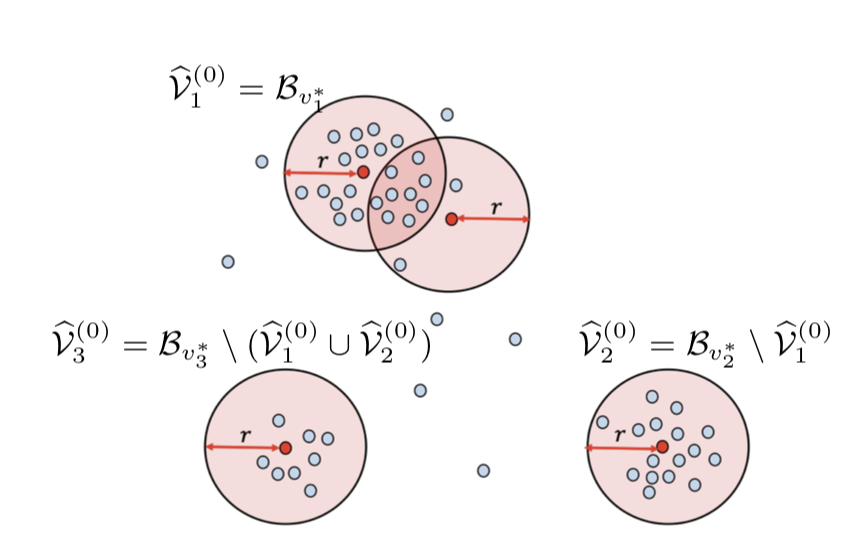
\includegraphics[width=.5\textwidth]{illustrate.png}
\end{figure}

\begin{prop}[Uniform approximation for single index tensor]\label{prop:approximation} Consider $\tT\in\caliT(d,s,m)$ and $f\in\calif(C)$.  There exists a set of basis tensors $\{\tB_{\ell,k}\colon (k,\ell)\in[d]\times\mathbb{N}\}$, such that, for every number of pieces $k\in[d]$ and degree $\ell\in\mathbb{N}$, we have
\[
\mnormSize{}{f(\tT)-\tB_{k,\ell}}\leq C\left( {k\over sm}\right)^{-(\ell+1)} \quad \text{and}\quad \rank(\tB_{k,\ell})\leq k^{s}\ell^s.
\]
\end{prop}


The following is the key property of single index matrix by taking $k\gtrsim \Omega(sm)$ and $\ell=r^{1/s}k^{-1}$ in Proposition~\ref{prop:approximation}.
\begin{thm}[Dimension-free approximation error]\label{thm:approximation} Consider a single index tensor $\Theta=f(\tT)$, where $\tT\in \caliT(d,s,m)$ and $f\in\calif(C)$. For every rank $r\in\mathbb{N}_{+}$,  we have
\[
{1\over d^m}\FnormSize{}{\Theta-\textup{Proj}_r(\Theta)}^2 \lesssim C^2\exp\left(-{r^{1/s}\over sm}\right).
\]
The bound is uniform over $\tT\in\caliT(d,s,m)$ and $f\in\calif(C)$. 
\end{thm}

\begin{cor}[Nice smooth tensor model is of $\log$ rank] For any fixed $\varepsilon>0$, we have
\[
\rank_{\varepsilon}(\Theta):=\min\{\rank(\tA)\colon \mnormSize{}{\tA-\Theta}\leq \varepsilon\}\lesssim \log^s d.
\]
\end{cor}

\begin{cor}[Block tensor model with diverging number of blocks] Let $\Theta$ be a block tensor with $s$ blocks on each mode. The $\varepsilon$-rank of $\Theta$ is no more than
$r=\log d$. 
\end{cor}

When $f(x)=x$, $\rank(\Theta)=o(1)$. When oscillating $f(x)=\sin(x)$, ....? When monotonic $f(x)={\exp(-x)\over 1+\exp(-x)}$ at bounded regime $[a,b]$; $f$ is quantile transformation??

Why do we define domain on $[-1,1]$??

Marginal quantile transformed tensor estimation. Low rank. Order-preserving Transformed. Analogy of distance matrix??? 

Connection to sign-representable tensor. Require $f$ to be monotonic. Here smooth $f$ suffices...
\section{Single index model estimation for matrices}
%\begin{lem}[Atom matrices] Let $\mA$ be a rank-$s$ matrix. For every natural number $\ell\in\mathbb{N}_{\geq 0}$, we have
%\[
%\rank(\mA^{\circ \ell})\leq {\ell+s-1 \choose s-1}.
%\]
%\end{lem}

%Given a latent factor $\mx=(x_1,\ldots,x_s)\in \mathbb{R}^s$ with $\vnormSize{}{\mx}\leq 1$, we define the nominal mapping up to degree $\ell$,
%\[
%\Phi_\ell(\mx)=(1,x_1,\ldots,x_s,x^2_1,x_1x_2,\ldots,x^2_s,\ldots,x^{\ell}_1,\ldots,x^{\ell}_s).
%\]
%Note that the covering number of $s$-dimensional bounded set $\tX$ is $\tN(1/k, \tX, \mnormSize{}{\cdot})\leq k^s$. Let $\tE_k$ denote the corresponding covering set. Then,  $\tE_k$ satisfies 
%\begin{enumerate} 
%\item $|\tE_k| \leq k^s$;
%\item For every $\Delta \in\tE_k$, we have
%\[
% \max_{\mx_i,\mx_j\in \Delta}\mnormSize{}{\mx_i-\mx_j}\lesssim {1\over k}.
%\]
%\item $\Delta \cap \Delta'=\emptyset$ for all $\Delta\neq \Delta'\in\tE_k$.
%\end{enumerate}

%Now given $(\mx_i,\my_j)\in\tX\times\tX$, we define piece-wise polynomial matrix $\mA_{k,\ell}\in\mathbb{R}^{d\times d}$ with $k$-pieces and polynomial degree of $\ell$
%\[
%\mA_{k,\ell}(i,j)=\sum_{\Delta\in \tE_k}\langle \Phi_{\ell}(\mx_i), \mbeta_{\Delta}\rangle\mathds{1}\{\mx_i\in \Delta\}.
%\]
%\\
%\begin{prop}[Rank of Monomial Matrices] Let $\mA_{k,\ell}$ be the piecewise monomial matrix of degree up to $\ell$. Then,
%\[
%\rank(\mA_{k,\ell})\leq k^s\sum_{i=0}^\ell{\ell+s-1 \choose s-1} \leq k^s(\ell+s-1)^s.
%\]
%\end{prop}
%\begin{prop}[Uniform approximation of single index matrices] \label{thm:approximation}%Consider $z(i)=\lfloor {ik \over d} \rfloor$ for all $i\in[d]$. Define a $k$-block matrix $\mB$ with $(i,j)$-th entry
%\[
%\mB(i,j):=\mTheta(z(i),z(j)), \quad \text{for all }(i,j)\in[d]^2.
%\]
%Consider $\mTheta\in\tP(d,\alpha,s,L)$. For every natural integers $k\leq d$ and $\ell \leq \lfloor \alpha \rfloor$, there exists a matrix $\mA_{\ell,k}$ with $\rank(\mA_{k,\ell})\leq k^s\ell^s$ such that
%\begin{equation}
%\mnormSize{}{\mTheta-\mA_{k,\ell}}\lesssim L k^{-\ell}\ell^s.
%\end{equation}
%\end{prop}

%The following is the key property of single index matrix by taking $k\gtrsim \Omega(1)+1$ and $\ell=r^{1/s}k^{-1}$ in Theorem~\ref{thm:approximation}.
%\begin{thm}[Dimension-free approximate rate] Let $\mTheta\in\tP(d,s,L)$. For every rank $r\in\mathbb{N}_{+}$,  we have
%\begin{align}
%{1\over d^2}\FnormSize{}{\mTheta-\textup{Proj}_{r}(\mTheta)}^2\lesssim
%\begin{cases}
%L^2r^{-2\alpha/s}, & \text{when }f\in \tH(\alpha, L),\\
%L^2\exp(-r^{1/s}), & \text{when }f\in \tC^{\infty}(L).
%\end{cases}
%\end{align}
%\[
%{1\over d^2}\FnormSize{}{\mTheta-\textup{Proj}_{r}(\mTheta)}^2\lesssim L^2\exp(-r^{1/s}).
%\]
%\end{thm}
\subsection{Spectral method and matrix lasso are both nearly minimax}
We now consider two estimations. The first one is convex estimater
\[
\hat \mTheta= \argmin_{\Theta}\left\{\FnormSize{}{\mY-\mTheta}^2+\sqrt{d}\sigma\nnormSize{}{\mTheta}\right\},
\]
and the other is non-convex estimator $r=sm\log^{s} d$. 
The closed-form solution is
\[
\hat \mTheta=\sum_{i=1}^{d}(\lambda_i(\mY)-\sqrt{d}\sigma)_{+}\mathbf{u}^T_i\mathbf{v}_j.
\]
\subsection{Nonconvex }
\begin{thm}[Polynomial estimation of single index matrix] Let $\mTheta=f(\mT)$ with $\mT\in\caliT(d,s,2)$ and $f\in\calif(C)$.
\[
\FnormSize{}{\hat \mTheta-\mTheta}\lesssim  d^{-1}\log^s(d).
\]
\end{thm}

%\begin{thm}[Polynomial estimation of single index matrix]
%\[
%\FnormSize{}{\hat \mTheta-\mTheta}\lesssim 
%\begin{cases}
%d^{-{2\alpha \over 2\alpha+s}}, \quad \text{when }f\in \tH^\alpha(L),\\
%d^{-1}\log^s(d), \quad \text{when }f\in \tC^{\infty}(L).
%\end{cases}
%\]
%\end{thm}

\begin{thm}[Minimax for matrices] Assume $s\asymp \tO(1)$. Denote the class $\calif \circ \caliT=\{\Theta: \Theta=f(\mT) \text{ for some }(\mT,f)\in\caliT(d,s,2)\times \calif(C)\}$. Then, when we have
\[
\inf_{\hat \Theta}\sup_{\mTheta\in \calif\circ \caliT}\mathbb{P}\left(\tR(\mTheta,\  \hat \mTheta)\gtrsim d^{-1}\right)\geq 0.2.
\]
\end{thm}
\begin{proof} For every $\alpha_1\leq \alpha_2\in(0,\infty)$
\[
\tP(d,\alpha_1,s,L)\supset \tP(d,\alpha_2,s,L)\supset  \cdots \tP(d,\infty,s,L) \supset \{\Theta\colon \rank(\Theta)\leq s\}.
\]
\end{proof}
Open question: Can we show sharper lower bound for $\alpha\neq\infty$? Graphon???
%\subsection{Extension to missing values}

%\[
%\FnormSize{}{\hat \Theta-\Theta}\lesssim \min_{r\in[d]} {ds\over d^2}+\exp(-r^{1/s})
%\]
\section{Tensor estimation }


\subsection{Non-convex double spectral algorithm}

\begin{thm}[Polynomial algorithm] low-rank approximation is substantially better. 
\begin{align}
\tR(\hat \mTheta,\mTheta)\leq
\begin{cases}
r^{m}+d^{m/2}r+d^mr^{-2\alpha}& r^{-2\alpha}\leq d^{-(m-1)},\\
\min(d^{{-{m\over 2}+{(m-\alpha-1)m\over 2\alpha}}},1) &  \alpha\leq {(m-1)^2\over m},\ r\asymp \min(d^{(m-1)/2\alpha},d)\\
d^{-{{m\over 2}+{m-1\over 2\alpha}}}& \alpha\geq {(m-1)^2\over m}, \ r\asymp  d^{m-1\over 2\alpha}\leq d^{m\over 2(m-1)}\\
d^{-{m\over 2}}\log d & \alpha=\infty, \ r\asymp \log d
\end{cases}
\end{align}
\end{thm}

Block approximation (bottleneck: truncate at $\alpha=1$):
\begin{align}
\tR(\hat \mTheta,\mTheta)\leq
\begin{cases}
d^{-{2\alpha m \over m+2\alpha}} & \alpha\leq 1\\
d^{-{2m \over m+2}}& \alpha\geq 1
\end{cases}
\end{align}


\begin{thm}[Minimax optimality for tensors] 
Order-$m$ with known design (bottleneck: truncate at $d^{-(m-1)}$ with unknown design)
\begin{align}
\tR(\hat \mTheta,\mTheta)\leq
\begin{cases}
d^{-{2\alpha m \over m+2\alpha}} & \alpha\leq {m(m-1)\over 2}\\
d^{-{(m-1)}}\log d& \alpha\geq {m(m-1)\over 2}
\end{cases}
\end{align}
\end{thm}

\subsection{Statistical and Computational Trade-offs}

%\begin{proof}
%\[
%|\{a_1+\ldots + a_r = k\colon a_s\in\mathbb{N}_{\geq 0}\}|
%\]
%\end{proof}

% Acknowledgments---Will not appear in anonymized version
\acks{Funding here.}

Can we apply tensor algorithm to matrices??
\section{Nice tensor model has $\log d$ rank}


\bibliography{yourbibfile}

\appendix
\section{Proof of Proposition 1}
\begin{proof}
By definition $\tT\in\caliT(d,s,m)$, $\rank(\Mat(\tT))\leq r$. Therefore, there exists matrix SVD such that
\[
\Mat(\tT)=\sum_{i\in[s]} \lambda_i\ma_i\otimes \mb_i,
\]
where $\ma_i\in\mathbb{R}^d$, $\mb\in\mathbb{R}^{d^{m-1}}$, and $\lambda_1\geq \cdots \lambda_s\geq 0$. By definition
\begin{align}\label{eq:svd}
\Mat(\tT^{\circ \ell})&=\left[\Mat(\tT)\right]^{\circ \ell}=\left(\sum_{i\in[s]}\lambda_i\ma_i\otimes \mb_i\right)^{\circ \ell}\\
&=\sum_{\substack{\kappa_1+\cdots+\kappa_s=\ell,\\ (\kappa_1,\ldots,\kappa_s)\in\mathbb{N}^s_{+}}}\lambda^{\kappa_1}_1\cdots\lambda^{\kappa_s}_s(\ma^{\circ \kappa_1}_1\circ \cdots \circ \ma^{\circ \kappa_s}_s)\otimes(\mb^{\circ \kappa_1}_1\circ \cdots \circ \mb^{\circ \kappa_s}_s).
\end{align}
Here $(\ma^{\circ \kappa_1}_1\circ \cdots \circ \ma^{\circ \kappa_s}_s) \in\mathbb{R}^{d}$ and $(\mb^{\circ \kappa_1}_1\circ \cdots \circ \mb^{\circ \kappa_s}_s)\in\mathbb{R}^{d-1}$. Now notice that by counting argument, 
\[
\#\{(\kappa_1,\ldots,\kappa_s) \in \mathbb{N}_{+}^{s} \colon \kappa_1+\cdots+\kappa_s=\ell\} = {\ell+s-1 \choose s-1}.
\]
Therefore, the summation~\eqref{eq:svd} consists of no more than ${\ell+s-1 \choose s-1}$ rank-1 terms. We conclude that
\[
\rank(\tT^{\circ \ell})=\text{rank}(\Mat(\tT^{\circ \ell}))\leq  {\ell+s-1 \choose s-1}.
\]
\end{proof}
\section{Proof of Lemma 2}
\begin{lem} we have
\[
\mnormSize{}{f(\tT)-\tB_{k,\ell}}\leq {\max_{|\eta|\leq 1}|f^{(\ell+1)}|(\eta)\over (\ell+1)!}\mnormSize{}{(\tT-\tO)^{\circ {\ell+1}}}\leq \left({k\over sm}\right)^{-(\ell+1)}. 
\]
\end{lem}
Note that the covering number of $s$-dimensional bounded set $\tX$ is $\tN(1/k, \tX, \mnormSize{}{\cdot})\leq k^s$. Let $\tE_k$ denote the corresponding covering set. Then,  $\tE_k$ satisfies 
\begin{enumerate} 
\item $|\tE_k| \leq k^s$;
\item For every $\Delta \in\tE_k$, we have
\[
 \max_{\mx_i,\mx_j\in \Delta}\mnormSize{}{\mx_i-\mx_j}\lesssim {1\over k}.
\]
\item $\Delta \cap \Delta'=\emptyset$ for all $\Delta\neq \Delta'\in\tE_k$.
\end{enumerate}
We label the center of the covering set by $\{\mo_1,\ldots,\mo_{k^s}\} \subset\{\mx_1,\ldots,\mx_d\}$. We use $z\colon [d]\to[k^s]$ to denote the membership of rows of $\mX$
\[
z(i)=\argmin_{j\in[k^s]}\mnormSize{}{\mx_i - \mo_j}, \quad\text{such that}\quad \mnormSize{}{\mx_i-\mo_{z(i)}}\leq {1\over k}.
\]
We define a block matrix $\tO\in(\mathbb{R}^{d})^{\otimes m}$ with entries
\[
\tO(i_1,\ldots,i_m)=\tC\times_1\mo_{z(i_1)}\times_2\cdots\times_m \mo_{z(i_m)} 
\]
Therefore
\[
\mnormSize{}{\tT-\tO}\leq \max_{(i_1,\ldots,i_m)\in[d]^m} |\tC\times_1 \mx_{i_1}\times_2\cdots \times_m \mx_{i_m}-\tC\times_1 \mo_{z(i_1)}\times_2\cdots \times_m \mo_{z(i_m)}|\lesssim mk^{-1}s^{1/2}.
\]
Define 
\[
\tB_{k,\ell}:=f^{(1)}(\tO)\circ (\tT-\tO)+{f^{(2)}(\tO)\over 2}\circ (\tT-\tO)^{\circ 2}+\cdots {f^{(\ell)}(\tO)\over \ell!} \circ (\tT-\tO)^{\circ \ell}.
\]
The membership partition $[d]^m$ into $k^{sm}$ blocks. We use $[d]^m=\cup_{n=1}^{k^{sm}}\Delta_n$ to denote these blocks. Within each block, the tensor $\tO$ takes the same value, 
\begin{align}
\tB_{k,\ell}(\omega)&=\KeepStyleUnderBrace{(a_{0,\Delta}+a_{1,\Delta}\tT+a_{2,\Delta}\tT^{\circ 2}+\cdots a_{\ell,\Delta} \tT^{\circ \ell})}_{:=\tI}\mathds{1}\{\omega\in \Delta \}.
\end{align}
%By the definition of $\tB$
%\[
%\Mat(\tB_{k,\ell})(i_1,i_{-1})=\sum_{j\in[k^s]} (a_{0,j,i_{-1}}+a_{1,j,i_{-1}}\Mat(\tT)+a_{2,j,i_{-1}}\Mat(\tT^{\circ 2})+\cdots a_{\ell,j,i_{-1}} \Mat(\tT^{\circ \ell}))\mathds{1}\{i_1\in\Delta_j\}.
%\]
Because there are $k^{s}$ blocks along mode 1, we conclude that
\[
\rank(\tB_{k,\ell})\leq k^{s} \sum_{n=1}^\ell{n+s-1 \choose s-1} \leq k^{s}(\ell+s-1)^s.
\]

\newpage
\section{My Proof of Proposition 1}
\begin{lem}[Polynomial and Unfolding]
Consider a function $f\colon (\mathbb{R}^s)^{\otimes m}  \to \mathbb{R}$. Suppose that, under $(\mathbb{R}^s)^{\otimes m} \cong \mathbb{R}^{sm}$, the function $f$ is a degree-$\ell$ polynomial of $(sm)$-variables; i.e. 
\[
g(\mx_1,\ldots,\mx_m)= \sum_{\kappa_1+\cdots+\kappa_{sm}\leq \ell}c(\kappa_{1},\ldots,\kappa_{sm}) x^{\kappa_{1}}_{11}\cdots x^{\kappa_{sm}}_{sm},
\]
where $x_{ij}$ denotes the $i$-th element in $\mx_j$, for $(i,j)\in[s]\times[m]$. 
Then the dimensional-$d$ order-$m$ tensor $\mG$ generated by $f$ and $(\ma_i)_{i\in[d]}$ admits
\[
\mG(i_1,\ldots,i_m)=g(\ma_{i_1},\ldots,\ma_{i_m}),\quad \text{for all}\ (i_1,\ldots,i_m)\in[d]^m.
\]
Then
\[
\rank(\mG) \leq \sum_{i=0}^\ell {i+s-1 \choose s-1}.
\]
\end{lem}
\begin{proof}
\[
\text{Unfold}(\mG)= 
\begin{bmatrix}
\Phi(\ma_1)\\
\vdots\\
\Phi(\ma_d)\\
\end{bmatrix}
\mB^T
=
\begin{bmatrix}
1& a_{11} & \cdots &a_{s1} &a^2_{11} & a_{11}a_{s1}& \cdots &a_{11}a_{21}a^{\ell-2}_{s1}\cdots & a^\ell_{s1} \\
\vdots\\
1& a_{1d} & \cdots &a_{sd} &a^2_{1d} & a_{1d}a_{1d}& \cdots &a_{1d}a_{2d}a^{\ell-2}_{sd}\cdots & a^\ell_{sd}
\end{bmatrix}
\mB^T
\]
\end{proof}


\begin{lem}[Uniform approximation] Consider $\Theta\in\tP(d,s,L)$. There exists a sequence of tensor $\{\tA_{\ell,k}\colon (k,\ell)\in[d]\times\mathbb{N}\}$ such that, for every number of pieces $k\in[d]$ and degree $\ell\in\mathbb{N}$, we have
\[
\mnormSize{}{\Theta-\tA_{k,\ell}}\leq Lk^{-\ell}\ell^{ms},\quad \text{and}\quad \rank(\tA_{k,\ell})\leq k^s\ell^s.
\]
\end{lem}
\begin{proof} Based on the definition of infinitely smooth function
\begin{align}
|\Theta-\tA_{k,\ell}|&\leq |f(\ma_{i_1},\ldots,\ma_{i_m})-g(\ma_{i_1},\ldots,\ma_{i_m})|\\
&\leq L\left(k\over a\right)^{-\ell}{\ell+ms-1\choose ms-1}\\
&\leq L\left(k\over a\right)^{-\ell} \ell^{ms}
\end{align}
\end{proof}

\begin{cor}[Nice tensor model is of $\log d$ rank] For any fixed $\varepsilon>0$, we have
\[
\rank_{\varepsilon}(\Theta):=\min\{\rank(\tA)\colon \mnormSize{}{\tA-\Theta}\leq \varepsilon\}\lesssim \log d.
\]
\end{cor}
Where does $d$ come from??
\begin{thm}[Dimension-free approximation] Let $\Theta\in\tP(d,s,L)$. For every rank $r\in\mathbb{N}_{+}$,  
\[
{1\over d^m}\FnormSize{}{\Theta,\ \text{Proj}_r(\Theta)}^2\lesssim L^2\exp(-c_0r^{1/s}).
\]
\end{thm}
\begin{proof}
Let $k=\Omega(2a)$ and $\ell=r^{1/s}k^{-1}$. Then
\[
\mnormSize{}{\Theta-\tA_{k,\ell}}\leq L 2^{-\ell}\ell^{ms} \lesssim L2^{-\ell}\asymp L\exp(-r^{1/s})
\]
\end{proof}
\section{My Proof of Theorem 2}

This is a complete version of a proof sketched in the main text.

\begin{lem}[Tensor polynomial approximation] Suppose that the function $f\colon [0,1]^m\to \mathbb{R}$ generating the signal tensor $\Theta$ is $\alpha$-H\"older smooth with $\alpha\in(0,\infty)$. Then, for any $k\geq d$, there exists a $k$-membership function $z\colon[d]\to[k]$ and a polynomial function such that
\[
\Theta(i_1,\ldots,i_K)- P_{\lfloor \alpha \rfloor}(\omega-\tS(z(i_1),\ldots,z(i_K))) \leq {m^2\over k^{\alpha}}
\],
\[
\mM(\mx-\mx_0)=
\begin{bmatrix}
1 &1&\cdots&1\\
x_1-x_0&x_2-x_0& \cdots &x_d-x_0\\
\vdots&\vdots&\vdots\\
(x_1-x_0)^{\lfloor \alpha \rfloor}&(x_2-x_0)^{\lfloor \alpha \rfloor}& \cdots &(x_d-x_0)^{\lfloor \alpha \rfloor}\\
\end{bmatrix}
\]
\end{lem}
%\[
%\tP=\{\tS, z \colon \Theta=\tS\times \mM\times\cdots \times \mM, \Theta=\Theta\otimes \math\}
%\]

\newpage
Let $z\colon[d]\to[k]$ denote the clustering function. For notational convenience, we use the shorthand $\mz(i_1,\ldots,i_m):=(z(i_1),\ldots,z(i_m))^T\in[k]^m$ to denote the block membership by applying $z$ to each of the $m$ modes. We make the convention that blockwise constant tensor is of degree 1 (not zero, for notational convenience).  
\begin{enumerate}
\item blockwise degree-$1$ (constant) tensor
\begin{align}
\tL(0,k)&=\left\{\tB\in(\mathbb{R}^{d})^{\otimes m}\colon \tB(i_1,\ldots,i_m)=\tC(z(i_1),\ldots,z(i_k)) \text{ for some tensor $\tC\in(\mathbb{R}^k)^{\otimes m}$}\right\}\\
&=\left\{\tB\in(\mathbb{R}^{d})^{\otimes m}\colon \Theta(\omega)= \sum_{\Delta \in[k]^m}c_{\Delta}\mathds{1}\{\mz(\omega)=\Delta\} \right\}\\
&\cong \{\tC \in\mathbb{R}^{k^m}, z\colon[d]\to[k]\}
\end{align}
where, for every cluster $\Delta\in[k]^m$, the coefficient $c_{\Delta}\in\mathbb{R}$ represents the mean within the cluster. We use $\tC=\{c_{\Delta}\colon \Delta\in[k]^m\}$ to collect all unknown coefficients. 

\item blockwise degree-$2$ linear tensor
\begin{align}
\tL(1,k)&=\left\{\tB\in(\mathbb{R}^{d})^{\otimes m}\colon \tB(\omega)=\sum_{\Delta \in [k]^m} \left[c_{\Delta}+\langle \boldsymbol{\beta}_{\Delta}, \omega\rangle\right] \mathds{1}\{\mz(\omega)=\Delta \}\right\}\\
&\cong\{\tC\in\mathbb{R}^{(1+m) \times k^m}, z\colon[d]\to[k]\}
\end{align}
where, for every cluster $\Delta\in[k]^m$, the coefficient $(c_{\Delta}, \boldsymbol{\beta}_{\Delta}) \in \mathbb{R}\times \mathbb{R}^d$ the mean and slope within the cluster. We use $\tC=\{(c_{\Delta}, \boldsymbol{\beta}_{\Delta})\colon \Delta\in[k]^m\}\cong\mathbb{R}^{(1+m)\times k^m}$ to collect all unknown coefficients. 


\item blockwise degree-$(\ell+1)$ polynomial tensor
\begin{align}
\tL(\ell+1,k)&=\left\{\tB\in(\mathbb{R}^{d})^{\otimes m}\colon \tB(\omega)=\sum_{\Delta \in [k]^m} \text{Poly}_{\ell,\Delta}(\omega) \mathds{1}\{\mz(\omega)=\Delta \}\right\}\\
&\cong\{\tC\in\mathbb{R}^{(\ell+m)^\ell\times k^m}, z\colon[d]\to[k] \}
\end{align}
where, for every cluster $\Delta\in[k]^m$, the coefficient $(c_{\Delta}, \boldsymbol{\beta}_{\Delta}) \in \mathbb{R}\times \mathbb{R}^d$ the mean and slope within the cluster. Note that the polynomial function $\text{Poly}_{\ell,\Delta}(\cdot)$ has at most $(\ell+m)^{\ell}$ unknown coefficients. We use $\tC \subset \mathbb{R}^{(\ell+m)^\ell \times k^m}$ to collect the unknown coefficients in the blockwise degree-$(\ell+1)$ polynomial tensor family. 


\end{enumerate}
Model:
\begin{align}\label{eq:model}
\Theta(i_1,\ldots,i_m)=f\left({\pi(i_1)\over d}, \ldots,{\pi(i_m)\over d}\right),\quad \text{for all }i_1<\cdots<i_d.
\end{align}
\begin{thm}(Blockwise polynomial tensor approximation) Suppose the function $f\colon[0,1]^m\to \mathbb{R}$ generating the signal tensor $\Theta$ as in model~\eqref{eq:model} is $\alpha$-H\"older smooth with $\alpha\in(0,\infty)$. Then, for every block size $k\leq d$ and degree $\ell\in\mathbb{N}_{+}$, we have the approximation error
%there exists a $k$-block degree-$\ell$ polynomial tensor $\tB\in\tL_\ell(k)$, such that
\[
\inf_{\tB\in \tL(\ell,k)}{1\over d^m}\FnormSize{}{\Theta-\tB}^2 \lesssim {m^2\over k^{2\min(\alpha,\ \ell)}}.
\]
\end{thm}

We propose the least-square estimate
\[
\hat \Theta^\textup{LSE}=\argmin_{\Theta\in \tL(\ell,k)}\FnormSize{}{\tY-\Theta}.
\]
Rigorously, the least-square estimate $\hat \Theta^\textup{LSE}$ is a family of estimates with tuning parameters $(\ell,k)$; we suppress the dependence on $(\ell,k)$ when no confusion arises. 

\begin{thm}[Least-square estimator] Let $\hat \Theta^\textup{LSE}$ denote the least-square estimate with degree $\ell^*=\lfloor \min(\alpha, {m(m-1)\over 2})\rfloor$ with block size $k^*=\lfloor d^{m\over m+2\ell^*} \rfloor$. Then, $\hat \Theta^\textup{LSE}$ obeys the error bound
\begin{equation}
\begin{aligned}
{1\over d^m}\FnormSize{}{\hat \Theta^\textup{LSE}-\Theta}^2&\lesssim 
\inf_{(\ell,k)\in\mathbb{N}_{+}\times[d]}\left\{{1\over k^{2\min(\alpha,\ell)}}+{k^m\ell^m \over d^{m}}+{\log d\over d^{m-1}}\right\}\notag \\
&\asymp
\begin{cases}
d^{-{2m\alpha \over m+2\alpha}} & \text{when }\alpha<m(m-1)/2,\\
 d^{-(m-1)}\log d & \text{when }\alpha\geq m(m-1)/2.\\
\end{cases}
\end{aligned}
\end{equation}
\end{thm}

\begin{thm}[Polynomial estimator] Suppose that the signal tensor $\Theta$ is generated in model~\eqref{eq:model} with $f\in \tH(\alpha)\cap \tM(\beta)$. Let $\hat \Theta^\textup{BC}$ be the estimator in with degree $\ell^*=\lfloor \min(\alpha, {m(m-1)\over 2})\rfloor$ and block size $k^*=\lfloor d^{m\over m+2\ell^*}\rfloor$. Then the estimator $\hat \Theta^{BC} $ satisfies
\[
{1\over d^m}\FnormSize{}{\hat \Theta^\textup{BC}-\Theta}^2\lesssim d^{-\beta(m-1)}}+
\begin{cases}
d^{-{2m\alpha \over m+2\alpha}} & \text{when }\alpha < m(m-1)/2,\\
 d^{-(m-1)}\log d & \text{when }\alpha \geq m(m-1)/2.\\
\end{cases}
\]
with very high probability. 
\end{thm}

\begin{rmk} For order-3 tensor with sufficiently smooth function $\alpha\geq 3$, the optimal choice of degree and block sizes is $(\ell^*, k^*)=(3,d^{1/3})$.
\end{rmk}

\begin{thm}[Minimax lower bound] For any given $\alpha\in(0,\infty)$, the problem of estimating $\alpha$-smooth tensors obeys the minimax lower bound 
\[
\mathbb{P}\left(\inf_{\hat \Theta}\max_{\Theta\in \tP(\alpha)} \FnormSize{}{\Theta-\hat \Theta}^2 \geq d^{-{2m\alpha\over m+2\alpha}}+d^{-(m-1)}\log d \right) >0.8.
\]
\end{thm}

\end{document}
